
\section{Acceleration of Gravity}

\makelabheader %(Space for student name, etc., defined in master.tex or labmanual_formatting_commands.tex)

\textbf{Objective} 

To determine the acceleration of gravity near the surface of the earth.

\textbf{Overview }

In a previous activity, you performed a video analysis of an object in free
fall to determine the equation of motion and to extract a value for the acceleration
of gravity near the surface of the earth. Now we will make a more accurate determination
of the acceleration of gravity by timing the motion of a freely falling object.
The ``picket fence'' has evenly spaced black bars on a piece
of clear plastic. When dropped through the photogate, the bars interrupt the
light beam. By measuring the distance between the bars, and using the time measurements
of the photogate, the acceleration of the freely falling picket fence can be
calculated. 

Apparatus 

\begin{itemize}
\item \textit{Science Workshop 750 Interface}
\item Photogate 
\item Picket fence 
\item \textit{DataStudio} software (Free Fall application)
\end{itemize}
Note: On using the ``Picket Fence''

\begin{enumerate}
\item When performing free-fall experiments, place a box with packing material under
the experiment to cushion the fall of the picket fence.
\item For accurate results drop the picket fence through the photogate vertically.
\item To achieve vertical alignment of the picket fence hold it between your thumb
and forefinger, centered at the top of the bar, before releasing.
\end{enumerate}
\textbf{Activity 1: Position and Velocity Graphs}

(a) Consider an object in free fall near the surface of the earth. Sketch your
predictions for the position \textit{vs.}~time and velocity \textit{vs.}~time graphs of the motion
of the object using dashed lines on the axes below. Assume that the positive
position axis is down.

\vspace{0.3cm}
{\par\centering 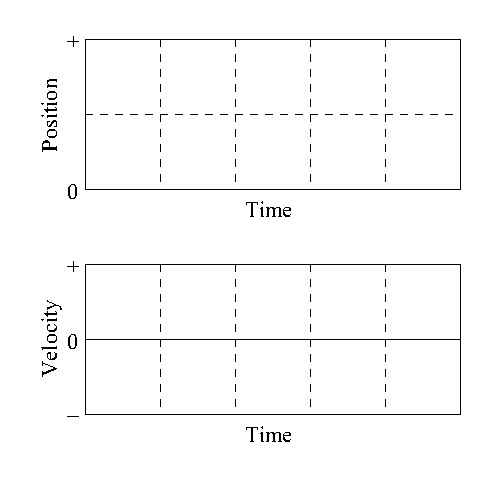
\includegraphics{acceleration/acceleration_fig1.eps} \par}
\vspace{0.3cm}

(b) Test your predictions by measuring the free fall of the picket fence. Open
the Free Fall application. Have one person hold the picket fence in a vertical
position above the gap between the arms of the photogate. Have another person
start recording data and then have the first person drop the picket fence through
the photogate. \textbf{Stop} the recording once the picket fence has passed
completely through the photogate. The computer will display graphs of position
versus time and velocity versus time. Sketch the results on the above axes using
solid lines.

(c) How do your predictions compare with the results of the measurements?
\vspace{20mm}

(d) What can you say about the magnitude and sign of the acceleration in this
case?
\vspace{20mm}

\textbf{Activity 2: Determining the Acceleration of Gravity }

(a) Fit the velocity \textit{vs.}~time graph to determine the acceleration. Repeat this
procedure to get a total of 20 good runs and record your results in a data table
below. For one of the runs, print the graph window and put a copy in your notebook
at the end of this unit.
\vspace{50mm}

(b) Use Excel to find the mean and standard deviation for the acceleration
measurements and record the results below in the form $g = \mbox{Mean}
\pm \sigma$.
\vspace{10mm}

(c) Compare your average acceleration with the standard value of 9.80 m/s\( ^{2} \).
This is done by calculating the \% difference. The \% difference is calculated
by subtracting the accepted value from your value, dividing by the accepted
value and multiplying by 100.
\vspace{20mm}

(d) Does your mean acceleration fall within one standard deviation of the accepted
value? Is there any indication of a systematic error? Explain.

